%---------------------------------------------------------------------------
% Chapter 2 - Related techonologies
%
%---------------------------------------------------------------------------
 
 
\section{Related technologies}


%---------------------------------------------------------------------------


%---------------------------------------------------------------------------
\subsection{GMA}
\label{ssec:gma}
GMA stands for Grid Monitoring Architecture~\cite{GMA1,GMA2}. It was originally introduced by Global Grid Forum in 2002. Need to create shared interface for monitoring grid resources emerged when several groups of researchers started working on systems facilitating grid monitoring and decided that those tools should be interoperable. System consists of three high level types of components of GMA which can be found in Figure~\ref{fig:gma}.

\begin{figure}[ht]
  \centering
  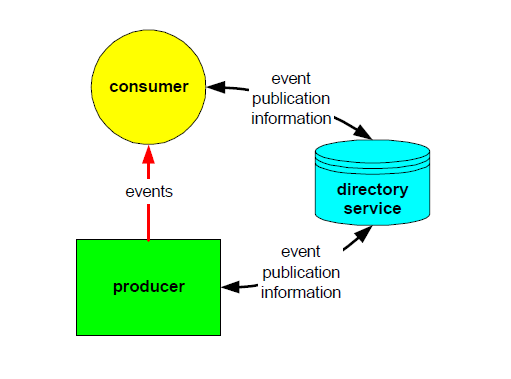
\includegraphics[width=0.5\textwidth]{gma}
  \caption{GMA Components}
  \label{fig:gma}
\end{figure}

GMA compatible systems should operate on data that are timestamped performance events. Such an events are typed collections of structured. Data flow is always in one direction - from a producer to consumer. On the other hand, directory service acts as mediator between them and it\rq{}s work is done directly after successful connection establishment. GMA supports two data exchange models - publish/subscribe (similar to CORBA Event Service) and query/response. What should also be noticed, communication may be initiated by both component types - either by producer or subscriber.


\subsection{OMIS}
\label{ssec:omis}
OMIS, On-Line Monitoring Interface Specification is another example of affords aiming at standardization and interoperability between grid monitoring tools. Work on this project was started in 1995, and continued up to 2003. As an outcome of this work, interface specification in three versions was created: OMIS 1.0\cite{OMIS1}, 2.0\cite{OMIS2} and 2.1.

The main purpose of this work is to define an interface that will allow communication between development tools (e.g. debuggers, performance analyzers or load balancers) and parallel programs running in distributed environments. The researches had three main goals to achieve, namely to define interface that will be extensive and complete to allow it\rq{}s usage in present tools, to allow extendability and usage in tools not known yet and to allow high adaptability to current and future programming paradigms (shared memory, remote procedure call or client/server).

To achieve those goals, authors introduced two sub-interfaces - one for communication between tool and program (monitor/program-interface) and between toll and monitors (tool/monitor-interface) with additional extension points. Illustration of this model can be found in Figure~\ref{fig:omis}. Additionally, OMIS supports only request/response communication model.

\begin{figure}[ht]
  \centering
  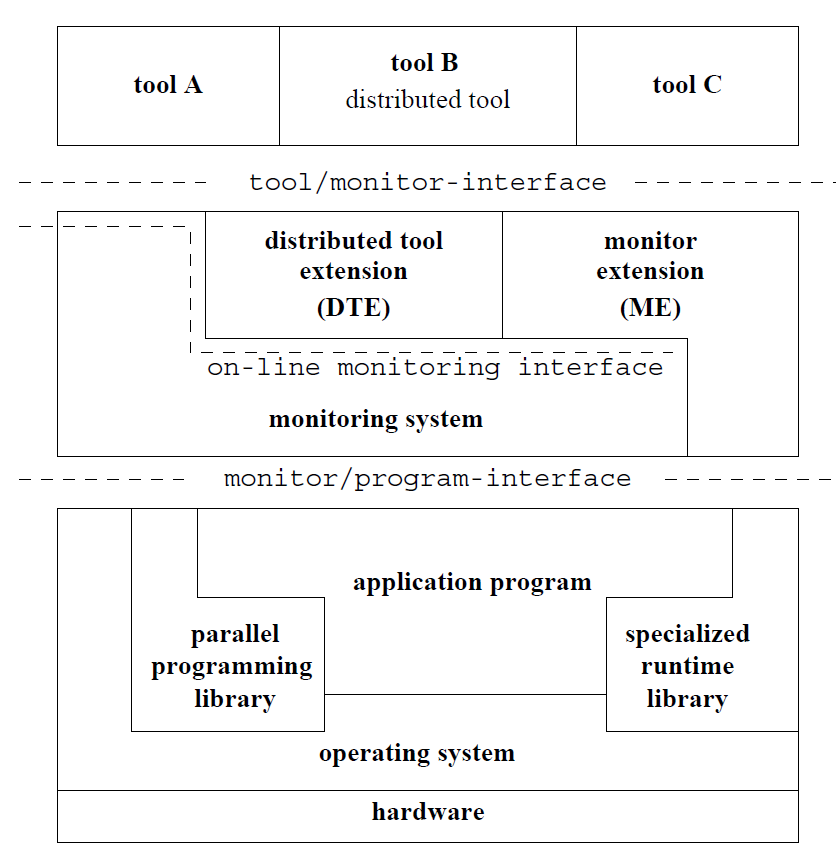
\includegraphics[width=0.7\textwidth]{omis}
  \caption{OMIS System Model}
  \label{fig:omis}
\end{figure}
  
      
